\chapter{Characterization \& Benchmarks}

  \section{Relative Object Size for Fully Structured Matrices} \label{sec:rel-object-size-fully-structured}

    In order to characterize the C3SR-format's storage scheme two families of matrices derived from structured grids are
    inspected. The matrices correspond to the 3-axial symmetric discretization of the Laplacian $\nabla^2 u(\vec{r}) =
    0$ over a structured cubic grid of edge size $d$ and correspond to a symmetric 7-point stencil operation, an
    example of which for $d = 5$ was shown previously and is reprinted here in Figure
    \ref{fig:laplacian-example-reprint} for convenience.

    Note that the matrices used in this section present ideal use cases around which the C3SR-format was conceived. The
    effects of deviations from this ideal will be explored in the next section by introducing perturbations to the
    regularity of the matrices.

    \begin{figure}[H]
        \centering
        \begin{minipage}{0.45\textwidth}
          \centering
          \input{fig/laplacian_example.tikz}
        \end{minipage}\hfill
        \begin{minipage}{0.45\textwidth}
          \centering
          \includegraphics[width=1.0\textwidth]{fig/laplacian_example.png} % second figure itself
        \end{minipage}
        \toccaption{Structured grid and corresponding matrix for a simple Laplacian.}{This example grid with
        an edge size of $d = 5$ is representative of the matric
        matrices used in Section \ref{sec:objsize-fully-structured}}
        \label{fig:laplacian-example-reprint}
    \end{figure}

    The CSR format's storage requirements are identical for both matrix families as they differ only in their nonzero's
    numerical values. Per nonzero one element is stored in the values array and in the column-index array in addition to
    one entry to the row-pointer array per matrix row. As for large matrices the vast majority of rows corresponds to
    inner nodes which all have $7$ nonzeros, or more formally, $\lim \limits_{d\rightarrow \infty}
    \frac{n_{\text{nnz}}}{n_{\text{row}}} = 7$. The number of rows can thus be expressed in terms of the number of
    nonzeros in the limit $d \rightarrow \infty$ and hence the storage requirements per nonzero amount to the following
    value:

    \begin{center}
      \begin{tikzpicture}
        \node[draw=dodgerblue4, inner sep=0.4cm, font=\Large] (EQ)
        {
          $
          \lim \limits_{d \rightarrow \infty}\frac{n_{\text{Bytes}}}{n_{\text{nnz}}}
          = \frac{\overbrace{(8 + 4) \cdot n_{\text{nnz}}}^{\text{V + CI}} + \overbrace{4 \cdot n_{\text{row}}}^{\text{RP}}}{n_{\text{nnz}}}
          = 12 + 4\cdot \lim \limits_{d \rightarrow \infty} \frac{n_{\text{nnz}}}{n_{\text{nrow}}}
          = 12 + \frac{4}{7}
          \approx 12.57
          $
        };
        \node[draw=dodgerblue4, fill=dodgerblue4, text=white, anchor=south west, inner sep=0.2cm] (WHAT)
          at (EQ.north west)
          {$1^{\text{st}}$ and $2^{\text{nd}}$ Matrix Family in CSR-Format};
      \end{tikzpicture}
    \end{center}

    In order to analyze the relative storage requirements of the corresponding objects in C3SR-format the sizes of the
    individual data arrays must be examined. By design, matrices with unique values produce one element per nonzero in
    the values array V. J encodes the unique adjacency patterns of the matrix's nodes and thus locks in at $135$ elements for
    any $d \geq 3$, produced by the $8$ corners a $4$ neighbors, $12$ edges a $5$ neighbors, $6$ faces a $6$ neighbors
    and the inner nodes with $7$ neighbors each. In smaller grids one or more unique node classes are not present.

    Every node in a contiguously indexed set of inner nodes produces a contiguous segment of $7$ unique values within V
    and hence the index-pointers $vs_i$ in VS increase at a fixed increment of $7$ for these nodes, which allows the
    segment within VS to be condensed into a single run-length-increment encoded triplet, as illustrated in Figure
    \ref{fig:rlei-encoding-of-vs}. The constant stride offset between the $d-2$ elements $vs_i$ is eventually
    interrupted at the grid's border where the corresponding matrix rows have fewer nonzeros. Thus, with exceptions
    arising at rows corresponding to nodes at the $y$- and $z$-borders, VS chiefly consists of blocks of two
    RLI-triplets: the first for a contiguous segment of $d-2$ inner nodes as explained above followed by another triplet
    encoding the two nodes at the $x=d-1$ and $x=0$ boundaries, prefacing the next contiguous segment of inner rows. In
    total, there are $(d-2)^2$ such block pairs. Consider Figure \ref{fig:laplacian-example-reprint} as an example: The
    first contiguous segment of inner rows comprises indices $\{32, 33, 34\}$ and is followed by the boundary nodes
    $\{35, 36\}$. The next contiguous segment then follows at index $37$ etc.

    \begin{figure}[H]
      \centering
      \captionsetup{width=0.9\textwidth}
      \begin{tikzpicture}[
        node distance=1cm and 0.1cm,
        vsstyle/.style={draw=gray, minimum height=1cm, minimum width=3cm, fill=dodgerblue4, text=white},
        vstyle/.style={draw=gray, minimum height=1cm, minimum width=3cm},
        pathstyle/.style={->}
      ]
        \node[circle, draw=gray] (VNAME)
          {V};
        \node[anchor=west, right=of VNAME] (DOTS1)
          {$\cdots$};
        \node[vstyle, right=of DOTS1, anchor=west] (VK)
          {$v_{k}$};
        \node[right=of VK, anchor=west] (DOTS2)
          {$\cdots$};
        \node[vstyle, right=of DOTS2, anchor=west] (VKP7)
          {$v_{k+7}$};
        \node[right=of VKP7, anchor=west] (DOTS4)
          {$\cdots$};
        \node[right=of DOTS4, anchor=west] (DOTS5)
          {$\cdots$};
        \node[vstyle, right=of DOTS5, anchor=west] (VKD)
          {$v_{k+7\cdot((d-1) - 2)}$};
        \node[right=of VKD, anchor=west] (DOTS6)
          {$\cdots$};

        \node[circle, anchor=center, fill=dodgerblue4, text=white, draw=gray] (VSNAME)
          at ($(VNAME)+(0,-2.0)$)
          {VS};
        \node[anchor=west] (VSDOTS1)
          at ($(VSNAME.east)+(0.5,0)$)
          {$\cdots$};
        \node[vsstyle, right=of VSDOTS1] (VSR)
          {$vs_r$};
        \node[vsstyle, right=of VSR] (VSRP1)
          {$vs_{r+1}$};
        \node[right=of VSRP1] (VSDOTSVSRP1)
          {$\cdots$};
        \node[vsstyle, right=of VSDOTSVSRP1] (VSRPDM2)
          {$vs_{r + ((d-1)-2)}$};
        \node[right=of VSRPDM2] (VSDOTSVSRPDM2)
          {$\cdots$};

        \node[anchor=north, text=dodgerblue4, inner sep=0.2cm, fill=gray!15, draw=dodgerblue4] (TRIPLET)
          at ($(VSDOTSVSRP1.south)+(0, -2)$)
          {$\big(r, k, 7\big)$};

        \draw[pathstyle] (VSR.north) |- ($(VSR.north)!0.5!(VK.south)$) -| (VK.south);
        \draw[pathstyle] (VSRP1.north) |- ($(VSRP1.north)!0.5!(VKP7.south)$) -| (VKP7.south);
        \draw[pathstyle] (VSRPDM2.north) |- ($(VSRPDM2.north)!0.5!(VKD.south)$) -| (VKD.south);
        \draw[] (TRIPLET.north) -- (VSR.south);
        \draw[] (TRIPLET.north) -- (VSRP1.south);
        \draw[] (TRIPLET.north) -- (VSRPDM2.south);
        \draw[] (TRIPLET.north) -- (VSRPDM2.south);
        \draw[shorten >= 0.2cm] (TRIPLET.north) -- (VSDOTSVSRP1.south west);
        \draw[shorten >= 0.2cm] (TRIPLET.north) -- ($(VSDOTSVSRP1.south west)!0.5!(VSDOTSVSRP1.south)$);
        \draw[shorten >= 0.2cm] (TRIPLET.north) -- (VSDOTSVSRP1.south);
        \draw[shorten >= 0.2cm] (TRIPLET.north) -- ($(VSDOTSVSRP1.south east)!0.5!(VSDOTSVSRP1.south)$);
        \draw[shorten >= 0.2cm] (TRIPLET.north) -- (VSDOTSVSRP1.south east);
      \end{tikzpicture}
      \toccaption{Section within V and VS pertaining to a contiguous segment of inner nodes for matrices from the second
        family.}{Pointer-index values $vs_i$ are indicated by arrows to the elements they point. Inner nodes yield matrix
        rows with 7 nonzeros and thus the corresponding section of VS comprises $d-2$ contiguous elements whose values
        increase at a constant stride of $7$. This constellation is efficiently condensed into a single
        run-length-increment encoded triplet.}
      \label{fig:rlei-encoding-of-vs}
    \end{figure}

    Similarly to the constellation created by contiguous inner nodes any set of contiguous nodes at the grid's faces or
    edges can be compressed into two or three RLI-triplets. However, as their number grows linearly with $d$ compared to
    $d^2$ for the grid's inner volume their effects become minute for larger $d$ and are of no consequence to
    convergence behavior.

    JS exhibits the very same structure as VS, consisting mainly of pairs of RLI-triplets which correspond to contiguous
    inner nodes. All inner nodes exhibit the same pattern, hence all corresponding $js_i$ point the same element in $J$,
    producing a single RLI-triplet followed by a second one for the two following border nodes. In contrast to $VS$,
    whose $vs_i$ exhibit a stride of $7$ between inner nodes, the $js_i$ exhibit no offset equal to a stride of $0$
    which thus allows them to be run-length-increment encoded in just the same manner. RS is subject to the very same
    reasoning as JS: Nodes in the inside of the grid produce slices of rows with $7$ nonzeros each, interrupted by nodes
    at the grid boundaries. 

    As exemplified in Figure \ref{fig:laplacian-example-reprint} nodes at any $z > 0$ are adjacent to another node
    situated below them in negative $z$-direction and thus the peg indices of two adjacent nodes at $z > 0$ are offset
    by $1$ carrying on for all following nodes. Hence the peg indices for all nodes with $z > 0$ are condensed into a
    single RLI-triplet. Similarly for $z = 0$ all nodes at $y > 0$ are stored by single RLI-triplet leaving, at worst,
    $d$ further triplets to be stored for the remainder of the matrix.
 
    Finally, the COMP array requires $\mathcal{O}(d^2)$ bytes due to reasoning analogous to that pertaining to VS, JS
    and RS: SIMD chunks across inner nodes all produce the same composition yielding a single RLI-triplet followed by
    disturbances of this regularity at the grid's boundaries, after which the next chunk of rows corresponding to inner
    nodes is arrived at.

    Collating the above results yields that none of the data arrays except V require storage size larger than
    $\mathcal{O}(d^2)$. As $n_{\text{nnz}} \rightarrow 7\cdot d^3$ for increasing $d$ the storage size per nonzero
    converges to 8 for the second family of matrices, which is characterized by fully unique nonzeros.

    \begin{center}
      \begin{tikzpicture}
        \node[draw=dodgerblue4, inner sep=0.4cm, font=\Large] (EQ)
        {
          $
          \lim \limits_{d \rightarrow \infty}\frac{n_{\text{Bytes}}}{n_{\text{nnz}}}
          = \frac{\overbrace{8 \cdot n_{\text{nnz}}}^{\text{V}} +
                  \overbrace{\mathcal{O}(1)}^{\text{J}} +
                  \overbrace{\mathcal{O}(d^2)}^{\text{VS}} +
                  \overbrace{\mathcal{O}(d^2)}^{\text{JS}} +
                  \overbrace{\mathcal{O}(d^2)}^{\text{RS}} +
                  \overbrace{\mathcal{O}(d)}^{\text{JP}} +
                  \overbrace{\mathcal{O}(d^2)}^{\text{COMP}}}{n_{\text{nnz}}}
          = 8
          $
        };
        \node[draw=dodgerblue4, fill=dodgerblue4, text=white, anchor=south west, inner sep=0.2cm] (WHAT)
          at (EQ.north west)
          {$2^{\text{nd}}$ Matrix Family in C3SR-Format};
      \end{tikzpicture}
    \end{center}

    Considering matrices from the first family, whose nonzeros are all identical, note that the total number of elements
    in V is limited by unique classes of nodes in the grid, just as described above for J. In the same manner the
    storage requirements for $V$ are constant for all $d > 3$ and thus in $\mathcal{O}(1)$. Due to this VS exhibits the
    same configuration as JS in the case layed out above. J, JP and RS remain unchanged while COMP retains its storage
    size requirements of $\mathcal{O}(d^2)$. The composition of SIMD chunks across inner nodes only changes its type
    according to the new data layout. Thus the relative storage requirements of matrices from the first family, whose
    nonzeros are all identical, converges towards $0$.

    \begin{center}
      \begin{tikzpicture}
        \node[draw=dodgerblue4, inner sep=0.4cm, font=\Large] (EQ)
        {
          $
          \lim \limits_{d \rightarrow \infty}\frac{n_{\text{Bytes}}}{n_{\text{nnz}}}
          = \frac{\overbrace{\mathcal{O}(1)}^{\text{V}} +
                  \overbrace{\mathcal{O}(1)}^{\text{J}} +
                  \overbrace{\mathcal{O}(d^2)}^{\text{VS}} +
                  \overbrace{\mathcal{O}(d^2)}^{\text{JS}} +
                  \overbrace{\mathcal{O}(d^2)}^{\text{RS}} +
                  \overbrace{\mathcal{O}(d)}^{\text{JP}} +
                  \overbrace{\mathcal{O}(d^2)}^{\text{COMP}}}{n_{\text{nnz}}}
          = 0
          $
        };
        \node[draw=dodgerblue4, fill=dodgerblue4, text=white, anchor=south west, inner sep=0.2cm] (WHAT)
          at (EQ.north west)
          {$1^{\text{st}}$ Matrix Family in C3SR-Format};
      \end{tikzpicture}
    \end{center}

    A measurement of the relative object size is displayed in \ref{fig:bytespernnz} for a wide range of values of $d$
    and both families of matrices, comparing the CSR- and C3SR-format.

    ?? FAZIT ?? Zero-overhead

    \begin{figure}[H]
      \centering
      \captionsetup{width=0.9\textwidth}
      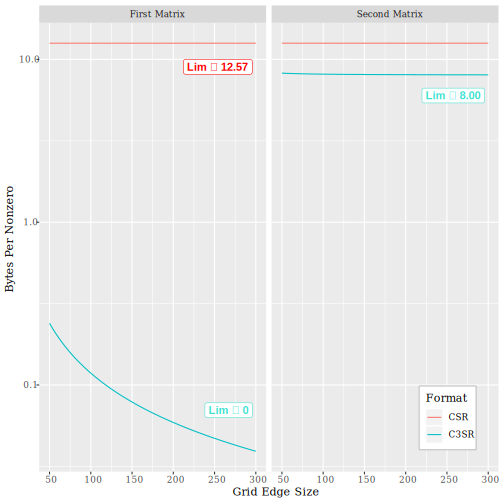
\includegraphics[width=0.9\textwidth]{assets/bytespernnz}
      \toccaption{Measured object storage size per nonzero matrix element for two families of sparse banded matrices derived from
        fully structured grids for the CSR- and C3SR-formats.}{Analytical convergence limits for $d \rightarrow \infty$
        are annotated next to each curve. The CSR's values are identical for both matrix families and the corresponding
        curve has been annotated only once. The matrix families correspond to the problem exemplified by Figure
        \ref{fig:laplacian-example} and differ only in the values of their nonzero elements, with the first family using
        a single constant value and the second family using unique values for each nonzero. Nonzeros are stored as
        8-byte double precision floats while indices are stored as 4-byte integers. Only values for $d \geq 50$ are
        displayed for the sake of legibility, as the overhead of the C3SR format's compression scheme yields very large
        relative storage size requirements for small matrices.}
      \label{fig:bytespernnz}
    \end{figure}

  \section{Object Size per Nonzero for Perturbed Structured Matrices}

    In contrast to the fully structured matrices examined in the previous section many real-life problems produce
    matrices whose structure exhibits deviations from the ideal in individual, non-contiguous rows. Such configurations
    may arise where the underlying mathematical problem entails integration over $1$- or $2$-dimensional manifolds in
    $3$-dimensional domains. These manifolds intersect the grid along nodes whose indexing is not contiguous introducing
    perturbations to the regularity of the resulting linear system's coefficient matrix at seemingly random positions of
    rows. See Figure \ref{fig:structured-grid-with-path} for an illustration of this notion.

    \begin{figure}[H]
      \centering
      \captionsetup{width=0.9\textwidth}

      \toccaption{Structured grid with integration path over non-contiguous nodes and corresponding matrix.}
        {?? 2D 10x10 Grid mit Integrationspfad und korresp. Matrix mit Störungen.}
      \label{fig:structured-grid-with-path}
    \end{figure}

    In order to gauge the stability of the C3SR-format's compression scheme to such configurations, which can be
    considered as slight deviations from the best-case scenario, the experiment performed in the previous section is
    repeated with perturbations introduced into the matrices. Choosing random matrix rows, their nonzeros' values and
    positions within the row are randomized. The values are drawn from a uniform distribution over the half-open
    interval $[1, 2)$ while the column indices are randomly selected from all possible column index values without
    duplication. Given a grid with edge size $d$ and its initial, unperturbed matrix the relative storage density as
    bytes per nonzero is measured while varying the relative ratio of matrix rows to perturb. The experiment is repeated
    to account for its stochastic aspect.

    Measurement results for two samples of matrices, based on a small and a larger grid, $d = 50$ and $d = 200$, and
    perturbations of up to $10\%$ of matrix rows are showcased in Figure \ref{fig:bytespernnz-perturbed}. Both families
    of matrices are shown to be very stable with respect to increasing ratios of perturbed rows. Matrices from the
    second family display a decrease in storage density of approximately $1\%$ per $1\%$ increase in the relative number
    of perturbed rows. A separate measurement reveals that the C3SR-format surpasses the CSR-format in storage density
    even if $75\%$ of matrix rows are randomized in the manner explained above and only the remaining $25\%$ are
    retained in their original, structured form. While matrices from the first family show a much greater decrease in
    storage density, their absolute values are very small, reaching approximately $2$ bytes per nonzero at $10\%$
    perturbed rows.  Except for different starting points of the unperturbed matrices, their underlying grid's size does
    not have any qualitative impact.

    \begin{figure}[H]
      \centering
      \captionsetup{width=0.9\textwidth}
      \includegraphics[width=0.9\textwidth]{assets/bytespernnz-perturbed}
      \toccaption{Measured object storage size per nonzero matrix element for two families of sparse banded matrices derived from
        fully structured grids for the CSR- and C3SR-formats.}{The graphs display mean values over 1000 iterations for each
        degree of perturbation. All respective standard deviations are smaller than $1\%$ of their correpsonding mean
        values.}
      \label{fig:bytespernnz-perturbed}
    \end{figure}

    The decrease in storage density is owed to the fact that a perturbed row's column indices are randomized,
    effectively increasing the pattern array J by $7$ elements and, for the first family of matrices whose values array
    V is essentially empty, also adding $7$ new unique values to V. Due to the fact, that the second family of matrices'
    V array is by far the largest of all of its data arrays, and because V does not increase in size as the values are
    uncompressible in the first place, randomizing a row has less effect as for first family matrices, explaining the
    difference in the decrease in storage density. In addition, run-length-increment encoding of the structural
    information of contiguous rows corresponding to segments of contiguous inner nodes is inhibited by every randomized
    matrix row within the segment for both matrix families.

    In summary, the C3SR format's storage scheme has shown to be stable to small perturbations. ...

  \section{MVM}

  The matrix-vector multiplication performance of the C3SR format is measured in its CSR-like and vectorized implementations (see \ref{subsec:matrix-vector-multiplication-schemes}). Firstly, a baseline performance is established by comparing the matrix-vector multiplication performance of the C3SR format's CSR-like multiplication scheme introduced in \ref{subsubsec:basic-csr-like-multiplication-scheme} against the CSR format's performance on different sparse banded matrices derived from structured grids and on three different machines. Secondly, the C3SR format's baseline performance is compared against its vectorized counterpart introduced in \ref{subsubsec:vectorized-simd-multiplication-scheme}.

  The following subsection introduces the sparse banded matrices used for the performance benchmarks and their method of acquisition. Subsequently, the results of the performance benchmarks are discussed. Information on the machines used for the benchmarks can be found at the ASC infrastructure wiki\footnote{https://mp-force.ziti.uni-heidelberg.de/kmbeutel/personal-wiki/wikis/ASC-infrastructure} (the KNL was configured to 50\% hybrid mode). All benchmarks were run multi-threaded utilizing the machines' full hardware capabilities.

  \section{Generation of Sparse Banded Matrices as Test Matrices}

    For the purpose of gauging the arithmetic performance, test matrices are created. These matrices resemble the structure of the sparse banded matrices introduced above and are created by iterating through a 3D grid of fixed integral dimensions X, Y, Z and applying a given stencil operation which encodes the desired adjacency relationship of the grid. Nodes requested by the stencil but missing from the grid, i.e. nodes on the grid's outer borders, are omitted, i.e. their corresponding entries in the adjacency matrix carry a zero corresponding to Dirichlet-type boundary conditions.

    The matrix's non-zero entries' numeric values are obtained from evaluating a sinusoidal function at the geometric center point $\vec{r} = (x, y, z)$ inbetween the two nodes in question whereby each Cartesian component $x, y, z$ is scaled by its coordinate's span $X, Y, Z$. An additional offset serves to prevent that entries in the matrix correponding to adjacent nodes according to the stencil incidentally evaluate to 0. The function utilized is $$W(x,y,z; n_x, n_y, n_z) = 2 + \sum \limits_{d \in \{x,y,z\}} \sin{\frac{d}{d_{\text{max}}} \cdot \pi \cdot n_d} $$ where $n_x, n_y, n_z$ are periodicity parameters for each dimensions. The matrix in Figure \ref{fig:laplacian-example} has been created using this method.

    Note that $n_d = 0 \Leftrightarrow \partial_d W(\vec{r}) \equiv 0$, introducing a periodicity in the corresponding dimension $d$. This feature is utilized to control the periodicity in the matrix's values.

    For the purpose of this work two different sets of parameters are utilized generating two different matrices: A smaller matrix generated from a $100 \times 100 \times 100$ grid with the periodicities $n_x = n_y = n_z = 0$ and a second matrix based on the same grid but different periodicities $n_x = 1.1; n_y = 1.2; n_z = 1.3$. Both matrices are generated from a symmetric 7p-stencil operation. The matrices' structures are their grid's equivalent to the example shown in Figure \ref{fig:laplacian-example}.

    The first matrix's values are identical for all rows whose pattern is the same such that \V and \J contain the same small number of elements. The second matrix's rows' values are all unique and thus \V contains approximately $7 \cdot 100^3$ elements (Figure \ref{fig:matrix_stats}).

    \begin{figure}[ht]
      \centering
      \begin{tabular}{ l | c c }
          Array & First Matrix & Second Matrix       \\
        \hline                                       \\
        \V         & $135$          & $6940000$      \\
        \VS        & $1000000$      & $1000000$      \\
        \J         & $135$          & $135$          \\
        \JS        & $1000000$      & $1000000$      \\
        \JP        & $1000000$      & $1000000$      \\
        \RS        & $1000000$      & $1000000$      \\
        Total Size in C3SR format & $\approx 16$MB & $\approx 72$MB \\
        Total Size in CSR Format & $\approx 87$MB & $\approx 87$MB \\
        \hfill
      \end{tabular}
      \caption[Matrices in C3SR format used for matrix-vector multiplication benchmarking.]{\textbf{Matrices in C3SR format used for matrix-vector multiplication benchmarking.} Number of elements is displayed for each array. \V stores double-precision floating-points while all other arrays use 32 bit-wide integers. Additionally, the matrix's size in CSR representation is listed.}
      \label{fig:matrix_stats}
    \end{figure}

    Note that the two matrices share the same structure and thus their only difference is found in \V and \VS. Concerning the vectorized matrix-vector multiplication scheme the first matrix primarily utilizes scheme II (Figure \ref{fig:simd_scheme_diag_collated}) while the second matrix mainly relies on scheme I (Figure \ref{fig:simd_scheme_diag}). The matrices are generated using the asc::matrixgen C++ library\footnote{https://mp-force.ziti.uni-heidelberg.de/asc/AscMatrixGen}.

  \section{Performance of CSR-like Matrix-Vector Multiplication}

    The C3SR format's CSR-like matrix-vector multiplication scheme (referred to as \emph{baseline implementation} hereinafter; see \ref{subsubsec:basic-csr-like-multiplication-scheme}) is compared against its CSR format's pendant using the Eigen C++ library \cite{eigen:website} on three different machines using the sparse banded matrices introduced in the previous section. The results are displayed in Figure \ref{fig:baseline_arithmetic_performance}.

    \begin{figure}[!ht]
      \centering
      \includegraphics[width=0.9\textwidth]{assets/eigen_vs_c3sr_baseline}
      \caption[Performance comparison of the CSR format against the C3SR format on sparse banded matrices.]{\textbf{Performance comparison of the CSR format against the C3SR format on sparse banded matrices.} The means and sample standard deviations of $10$ samples à $10000$ consecutive matrix-vector multiplications are shown. As the CSR format's representation of the different matrices is identical except for differing numeric values the arithmetic performance is the same save for statistical variance. The triangular symbols denote the theoretical limits as determined by the quotient of the total amount of data involved in a matrix-vector multiplication and the system's theoretical memory bandwidth. Since the matrix storage sizes differ between the storage formats two different limits are displayed.}
      \label{fig:baseline_arithmetic_performance}
    \end{figure}

    By design of the C3SR format, it outperforms the CSR format in the order of magnitude of around $50\%$ irrespective of the machine. This is due to the reduction in the size of the representation of the matrices and the consequent improvement in data locality as the C3SR format's arithmetic is slightly more complex as discussed in \ref{subsubsec:basic-csr-like-multiplication-scheme}. Accordingly, the performance improvement is more pronounced for the first matrix, whose storage size is smaller, entailing speed-up factors of approximately 2, 13, and 3.

    Despite the clear performance benefits the above results have to be qualified further as the implementation of the C3SR format\footnote{https://mp-force.ziti.uni-heidelberg.de/shuell/c3srmatrix} uses a NUMA-aware memory allocation scheme for its data arrays, correctly distributing them across physical memory, suitable for the multi-socket systems utilized for the benchmarks. Conversely, the Eigen C++ library, a general purpose linear algebra and numerics framework, does not tailor its data fields' memory layout in such a way that might lead to performance penalties due to a data distribution inadequate for the access patterns of the multi-threaded arithmetic. Additionally, Eigen internally uses the multi-threading framework OpenMP \cite{openmp:website} which entails a dynamic overhead not present in the implementation of the C3SR format.

  \section{Performance of SIMD Matrix-Vector Multiplication}

    The C3SR format's vectorized multiplication scheme's performance is measured by comparing it against the baseline performance. The implementation of the vectorized multiplication scheme utilizes the explicit SIMD vectorization library UME::SIMD \cite{umesimd2017}. The results are displayed in Figure \ref{fig:arithmetic-performance}.

    \begin{figure}[!ht]
      \centering
      \includegraphics[width=0.9\textwidth]{assets/arithmetic_performance}
      \caption[Performance of C3SR vectorized matrix-vector multiplication scheme compared to baseline implementation.]{\textbf{Performance of C3SR vectorized matrix-vector multiplication scheme compared to baseline implementation.} The means and sample standard deviations of $10$ samples à $10000$ consecutive matrix-vector multiplications are shown. The triangular symbols denote the theoretical limits as determined by the quotient of the total amount of data involved in a matrix-vector multiplication and the system's theoretical memory bandwidth.}
      \label{fig:arithmetic-performance}
    \end{figure}

    Sparse matrix-vector multiplication is a memory-bound computation so that the efficacy of a vectorized arithmetic implementation depends very strongly on the amount of data that is required to be read from memory and whether the dynamic overhead involved in determining the applicable SIMD scheme is compensated by a speed-up in arithmetic. This fact is reflected in the measurements as for the second matrix the SIMD implementation is generally slower than the baseline implementation. Only for the first matrix a significant speed-up can be observed on every machine. However, this might be partly due to the fact that the second matrix's SIMD multiplication scheme is less performant as it involves strided loads from memory which might equate to regular gather operations on the hardware used for this benchmark (see \ref{subsubsec:vectorized-simd-multiplication-scheme}).

  \section{Further Considerations}

    By evidence of the performance benchmarks presented in the previous section the basis for the performance gain in the arithmetic of the C3SR format with respect to the CSR format for sparse banded matrices is the reduction of the matrix's total storage size in memory leading to big improvements in data locality during matrix-vector multiplication.

    The C3SR format's storage scheme is tailored to minimize the matrix' storage size in memory. However, depending on how the matrix object is created in memory, adhering to the storage scheme to its full extent may not be optimal as it might limit parallelism during object construction. The data arrays' contents are strongly coupled such that the workload cannot be trivially spread across multiple threads. Instead, it might be advisable to partition the matrix into equally sized slices whose independent C3SR objects can be created in parallel. Finally, these distinct C3SR objects corresponding to the matrix slices are then transformed into a singular object by concatenating the data arrays requiring that the index-pointer arrays are offset by the number of rows preceding their first matrix row.

    \begin{figure}[ht]
      \centering
      \includegraphics[width=0.9\textwidth]{assets/structured_grid_matrix_heap_size}
      \caption[C3SR matrix storage size depending on partition size.]{\textbf{C3SR matrix storage size depending on partition size.} Numeric values are stored using double precision floating-point numbers while all other arrays utilize 32 bit integers. A point of diminishing returns is reached at a partition size of around 1000, past which the storage size in memory does not shrink significantly. Thus, creating C3SR objects using partition sizes of 1000 and larger may yield a similar performance while speeding up the creation of the object. For comparison the corresponding CSR format's storage size is provided.}
      \label{fig:structured_grid_matrix_heap_size}
    \end{figure}

    In order to establish an estimate for an apt partition size Figure \ref{fig:structured_grid_matrix_heap_size} displays the total storage size depending on the partition size for the two matrices used for the performance benchmarks. It is evident that there exists a point of diminishing returns past whose partition size there is no significant gain in storage size reduction. This point is reached when the sizes of \V and \J, the two arrays responsible for the reduction in storage size for the C3SR format, fall significantly below the fixed sizes of the remaining arrays, which constitute a minimum to the storage size.

    Thus, the performance benefits of the C3SR format may be kept even when trading larger storage sizes in favor of the parallelizability of the application.

